\documentclass{article}
\usepackage{graphicx,subcaption,lineno}
\usepackage{amsmath, amsthm, amsfonts, amssymb}
\usepackage{multirow,microtype}
\usepackage{longtable}

\frenchspacing

%\renewcommand{\thefigure}{S\arabic{figure}}
%\renewcommand{\thetable}{S\arabic{table}}
\usepackage{newfloat}
\DeclareFloatingEnvironment[name={Supplementary Figure}]{suppfigure}

\setcounter{figure}{0}

\title{Corrected figures from \cite{Smits2015}}
\author{Peter D Smits}
\date{}

\begin{document}
\maketitle


\begin{figure}[h]
  \centering
  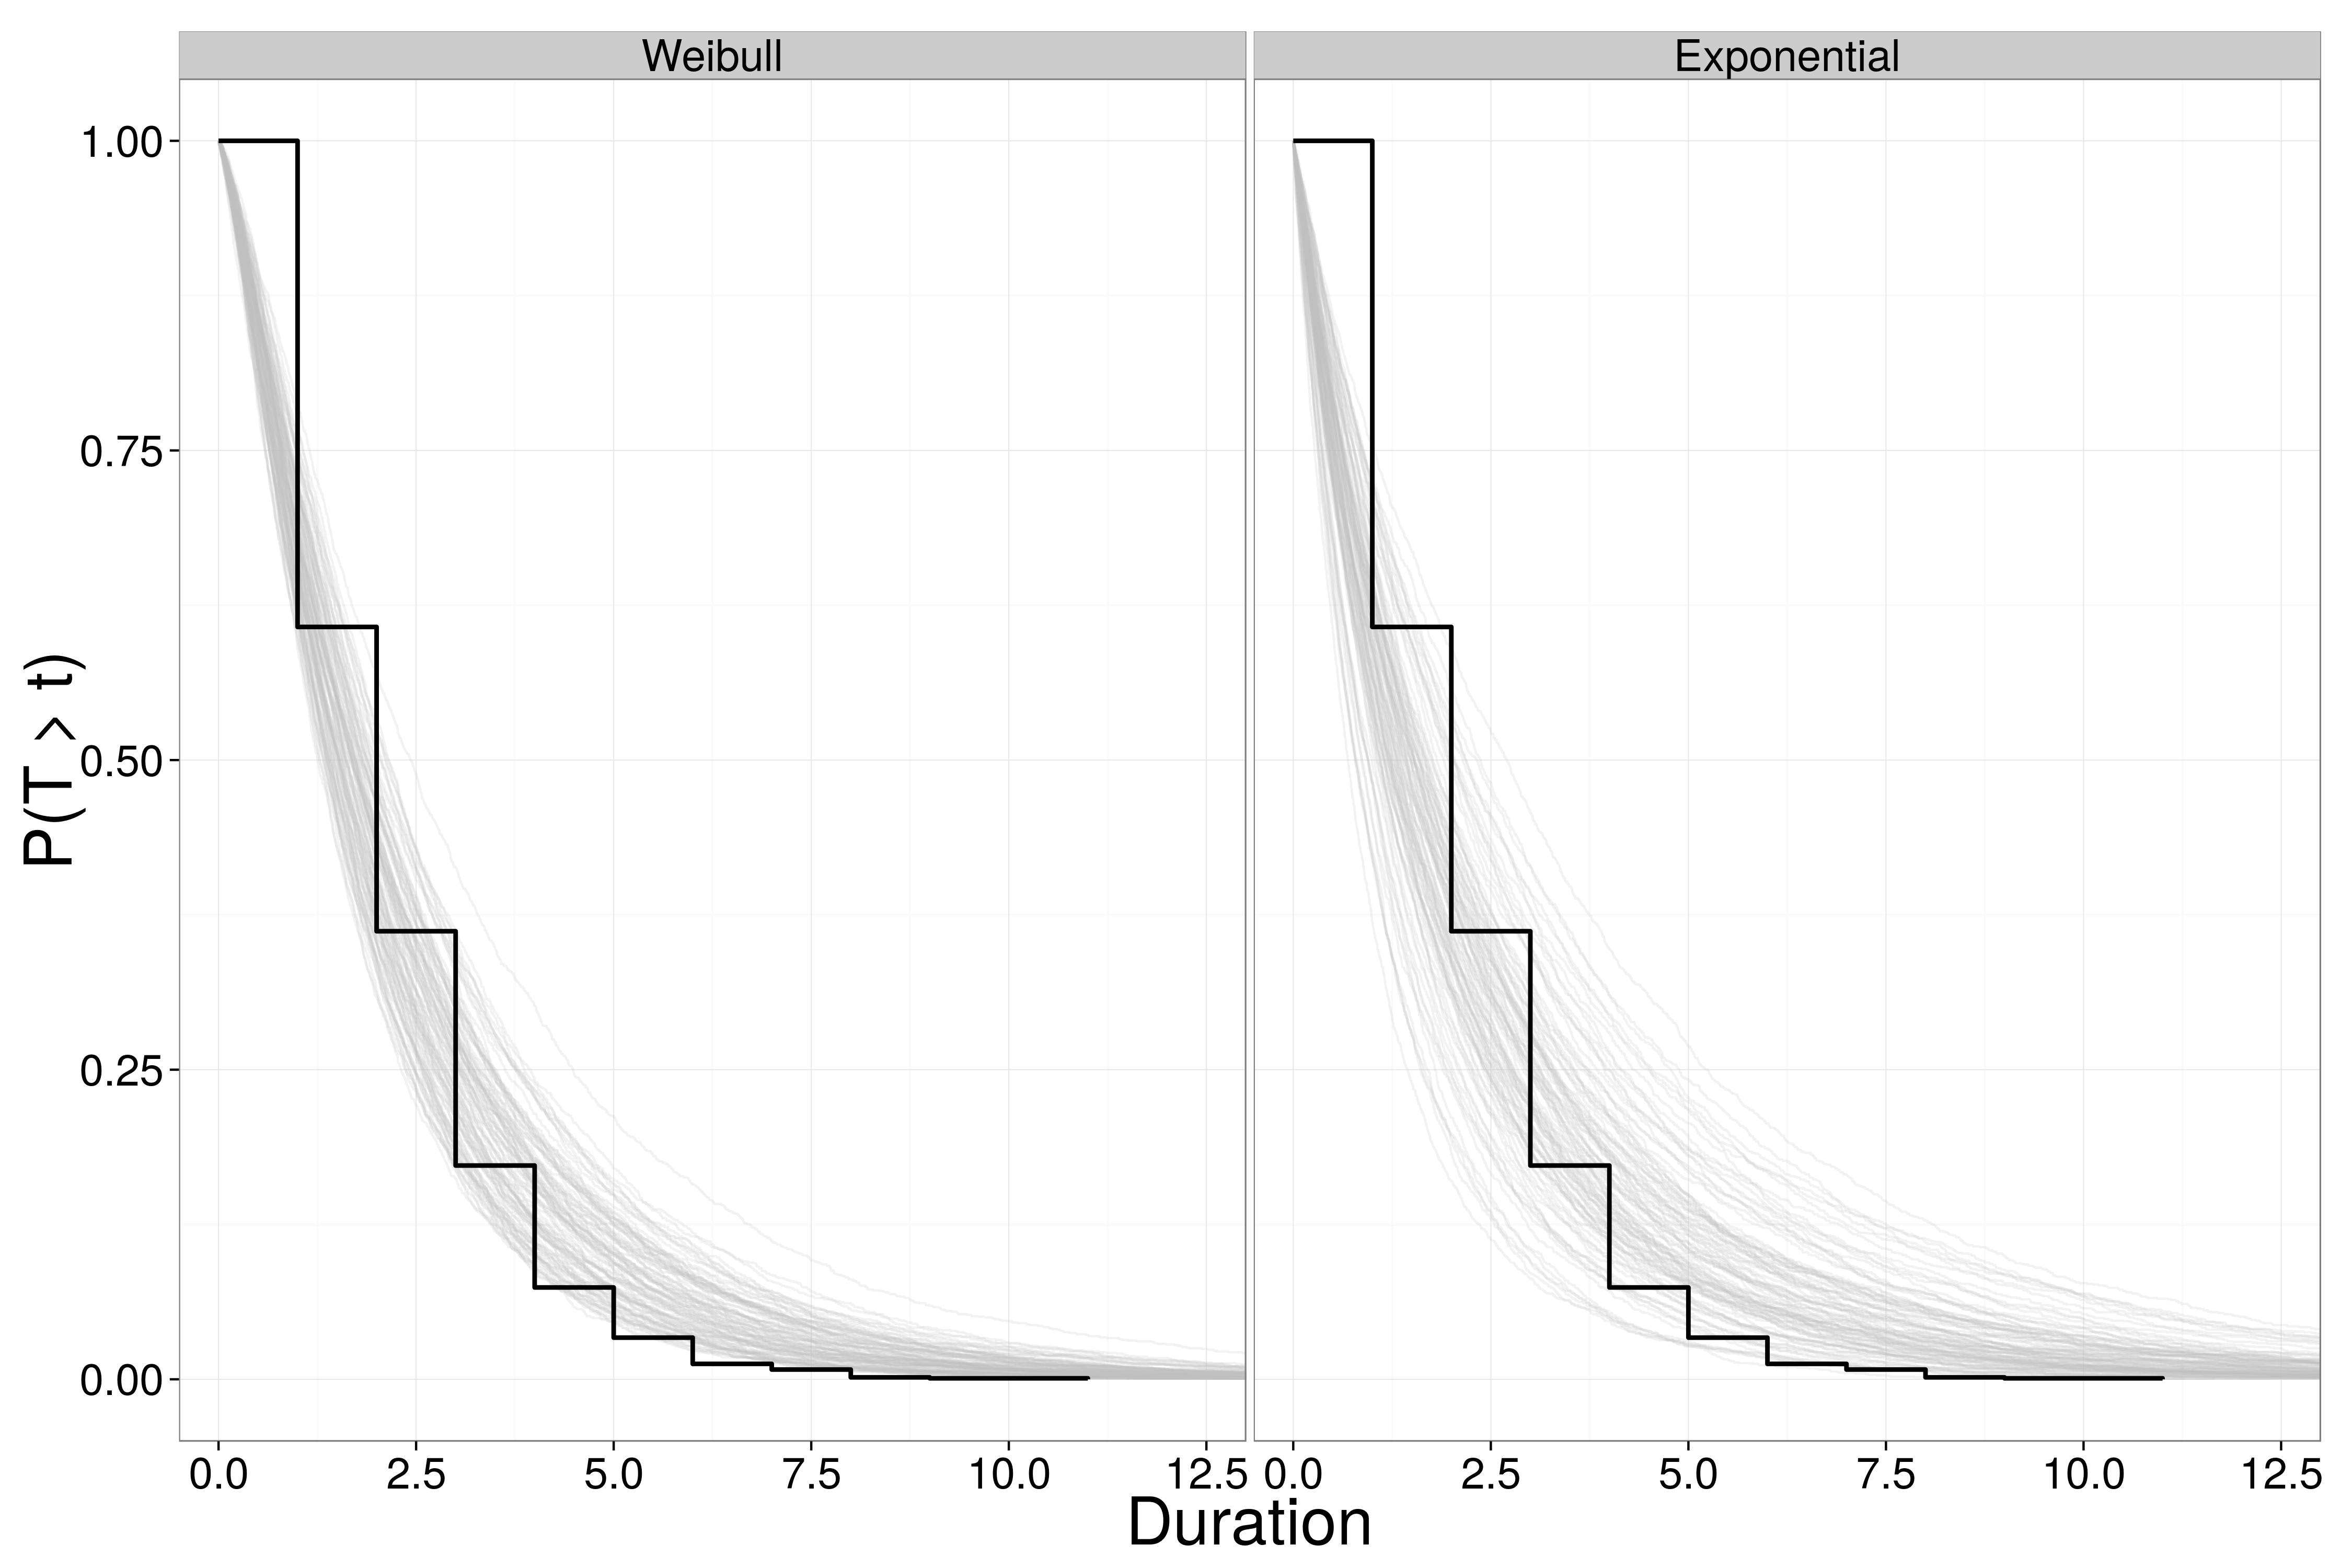
\includegraphics{figure/survival_function}
  \caption{Weibull-based model estimates (grey) from 1000 posterior predictive data sets of the empirical survival function (black). The survival function is the probability that a species with duration \(t\) will not have gone extinct. Simulated data sets were generated by drawing parameter values randomly from their estimated posteriors and using the observed covariate information to estimate durations for all the observed species.}
  \label{fig:ppc_surv}
\end{figure}
\clearpage

\begin{figure}[H]
  \centering
  \begin{subfigure}[b]{0.5\textwidth}
%    \caption{}
    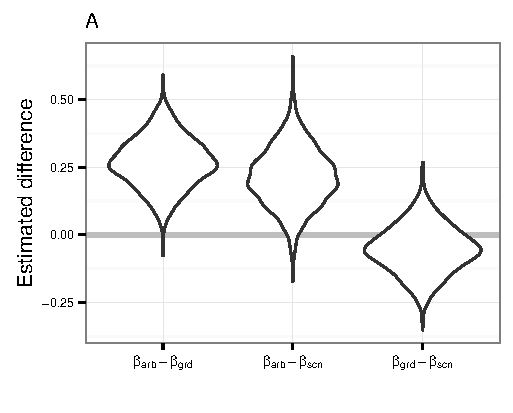
\includegraphics{figure/loco_diff_est}
%    \label{subfig:loco}
  \end{subfigure}
  \\
  \begin{subfigure}[b]{0.5\textwidth}
%    \caption{}
    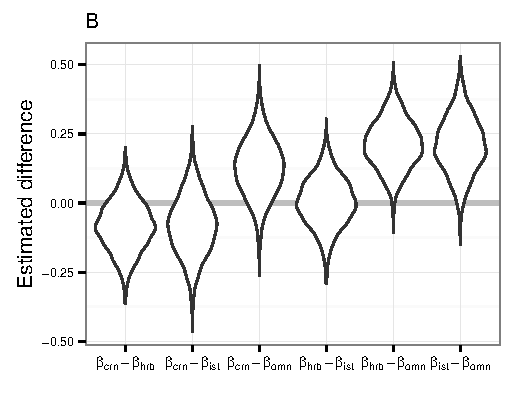
\includegraphics{figure/diet_diff_est}
%    \label{subfig:diet}
  \end{subfigure}
  \caption{Pairwise differences in effect of the locomotor (\textbf{A}) and dietary categories (\textbf{B}) on expected duration from 1000 samples from the posterior distribution. Comparisons of locomotor categories, from top to bottom (\textbf{A}), are: arboreal (\(\beta_{arb} = \beta_{0}\)) versus ground dwelling (\(\beta_{grd} = \beta_{0} + \beta_{g}\)), arboreal versus scansorial (\(\beta_{scn} = \beta_{0} + \beta_{s}\)), and ground dwelling versus scansorial. For dietary category, from top to bottom (\textbf{B}): carnivore (\(\beta_{crn} = \beta_{0}\)) versus herbivore (\(\beta_{hrb} = \beta_{0} + \beta_{h}\)), carnivore versus insectivore (\(\beta_{ist} = \beta_{0} + \beta_{i}\)), carnivore versus omnivore (\(\beta_{omn} = \beta_{0} + \beta_{o}\)), herbivore versus insectivore, herbivore versus omnivore, and insectivore versus omnivore. Negative values indicate that the first category is expected to have a greater duration than the second, while positive values indicate that the first category is expected to have a shorter duration.}
  \label{fig:trait_est}
\end{figure}
\clearpage


\begin{figure}[H]
  \centering
  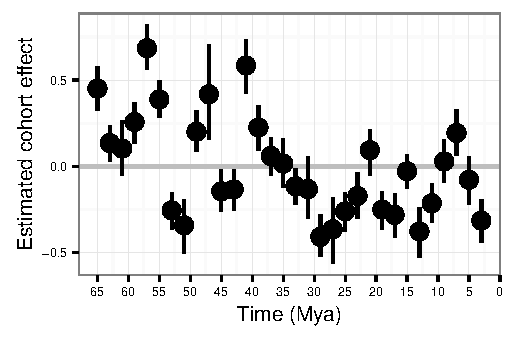
\includegraphics{figure/cohort_est}
  \caption{Summaries of posterior estimates of individual cohort effect depicted as medians and 80\% credible intervals. High values correspond to shorter species durations while lower values correspond to greater species durations compared to the mean duration. Lines are placed at the middle of the 2 My origination cohorts.}
  \label{fig:eff_cohort}
\end{figure}
\clearpage


\begin{figure}[H]
  \centering
  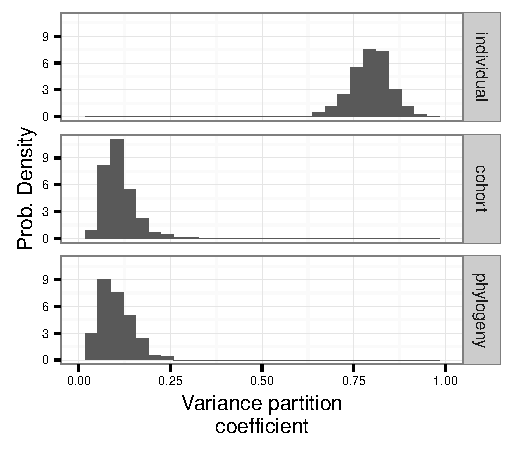
\includegraphics{figure/variance_est}
  \caption{Estimates of the variance partitioning coefficients for the three different sources of variance: species, cohort, and phylogeny. Higher values correspond to greater contribution to total observed variance. Each of the estimates is a distribution of 1000 approximating simulations due to the model's non-normally distributed errors.}
  \label{fig:vpc}
\end{figure}
\clearpage



\setcounter{figure}{0}


\begin{suppfigure}[h]
  \centering
  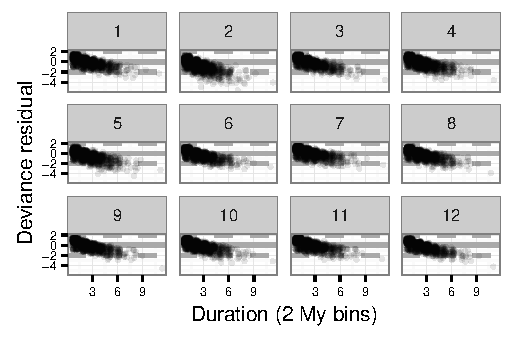
\includegraphics[height = 0.5\textheight, width = \textwidth, keepaspectratio = true]{figure/residual_plot}
  \caption{Deviance residuals from the fitted survival model compared to observed durations. Each graph depicts the residuals from single draws from the posterior distributions of all estimated parameters. Positive values indicate an underestimate of the observed duration, while negative values indicate an overestimate of the observed duration. A small amount of noise is added to each point to increase clarity. Twelve different examples are provided here to indicate consistency across multiple realizations.}
  \label{fig:ppc_res}
\end{suppfigure}

\begin{suppfigure}[h]
  \centering
  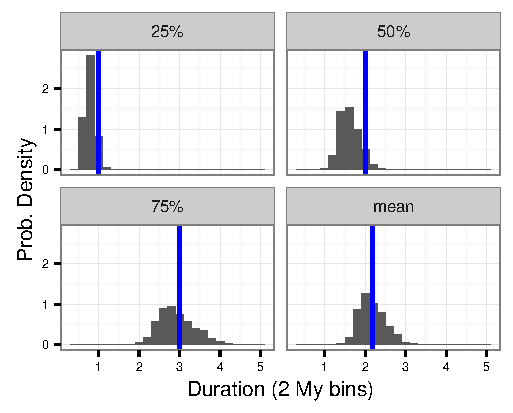
\includegraphics[height = 0.5\textheight, width = \textwidth, keepaspectratio = true]{figure/quant_ppc}
  \caption{The results of additional posterior predictive checks for four summaries of the observed durations, as labeled. Blue vertical lines indicate the observed value. None of the observed values are significantly different from the posterior predictive distributions.}
  \label{fig:ppc_quant}
\end{suppfigure}

\begin{suppfigure}[h]
  \centering
  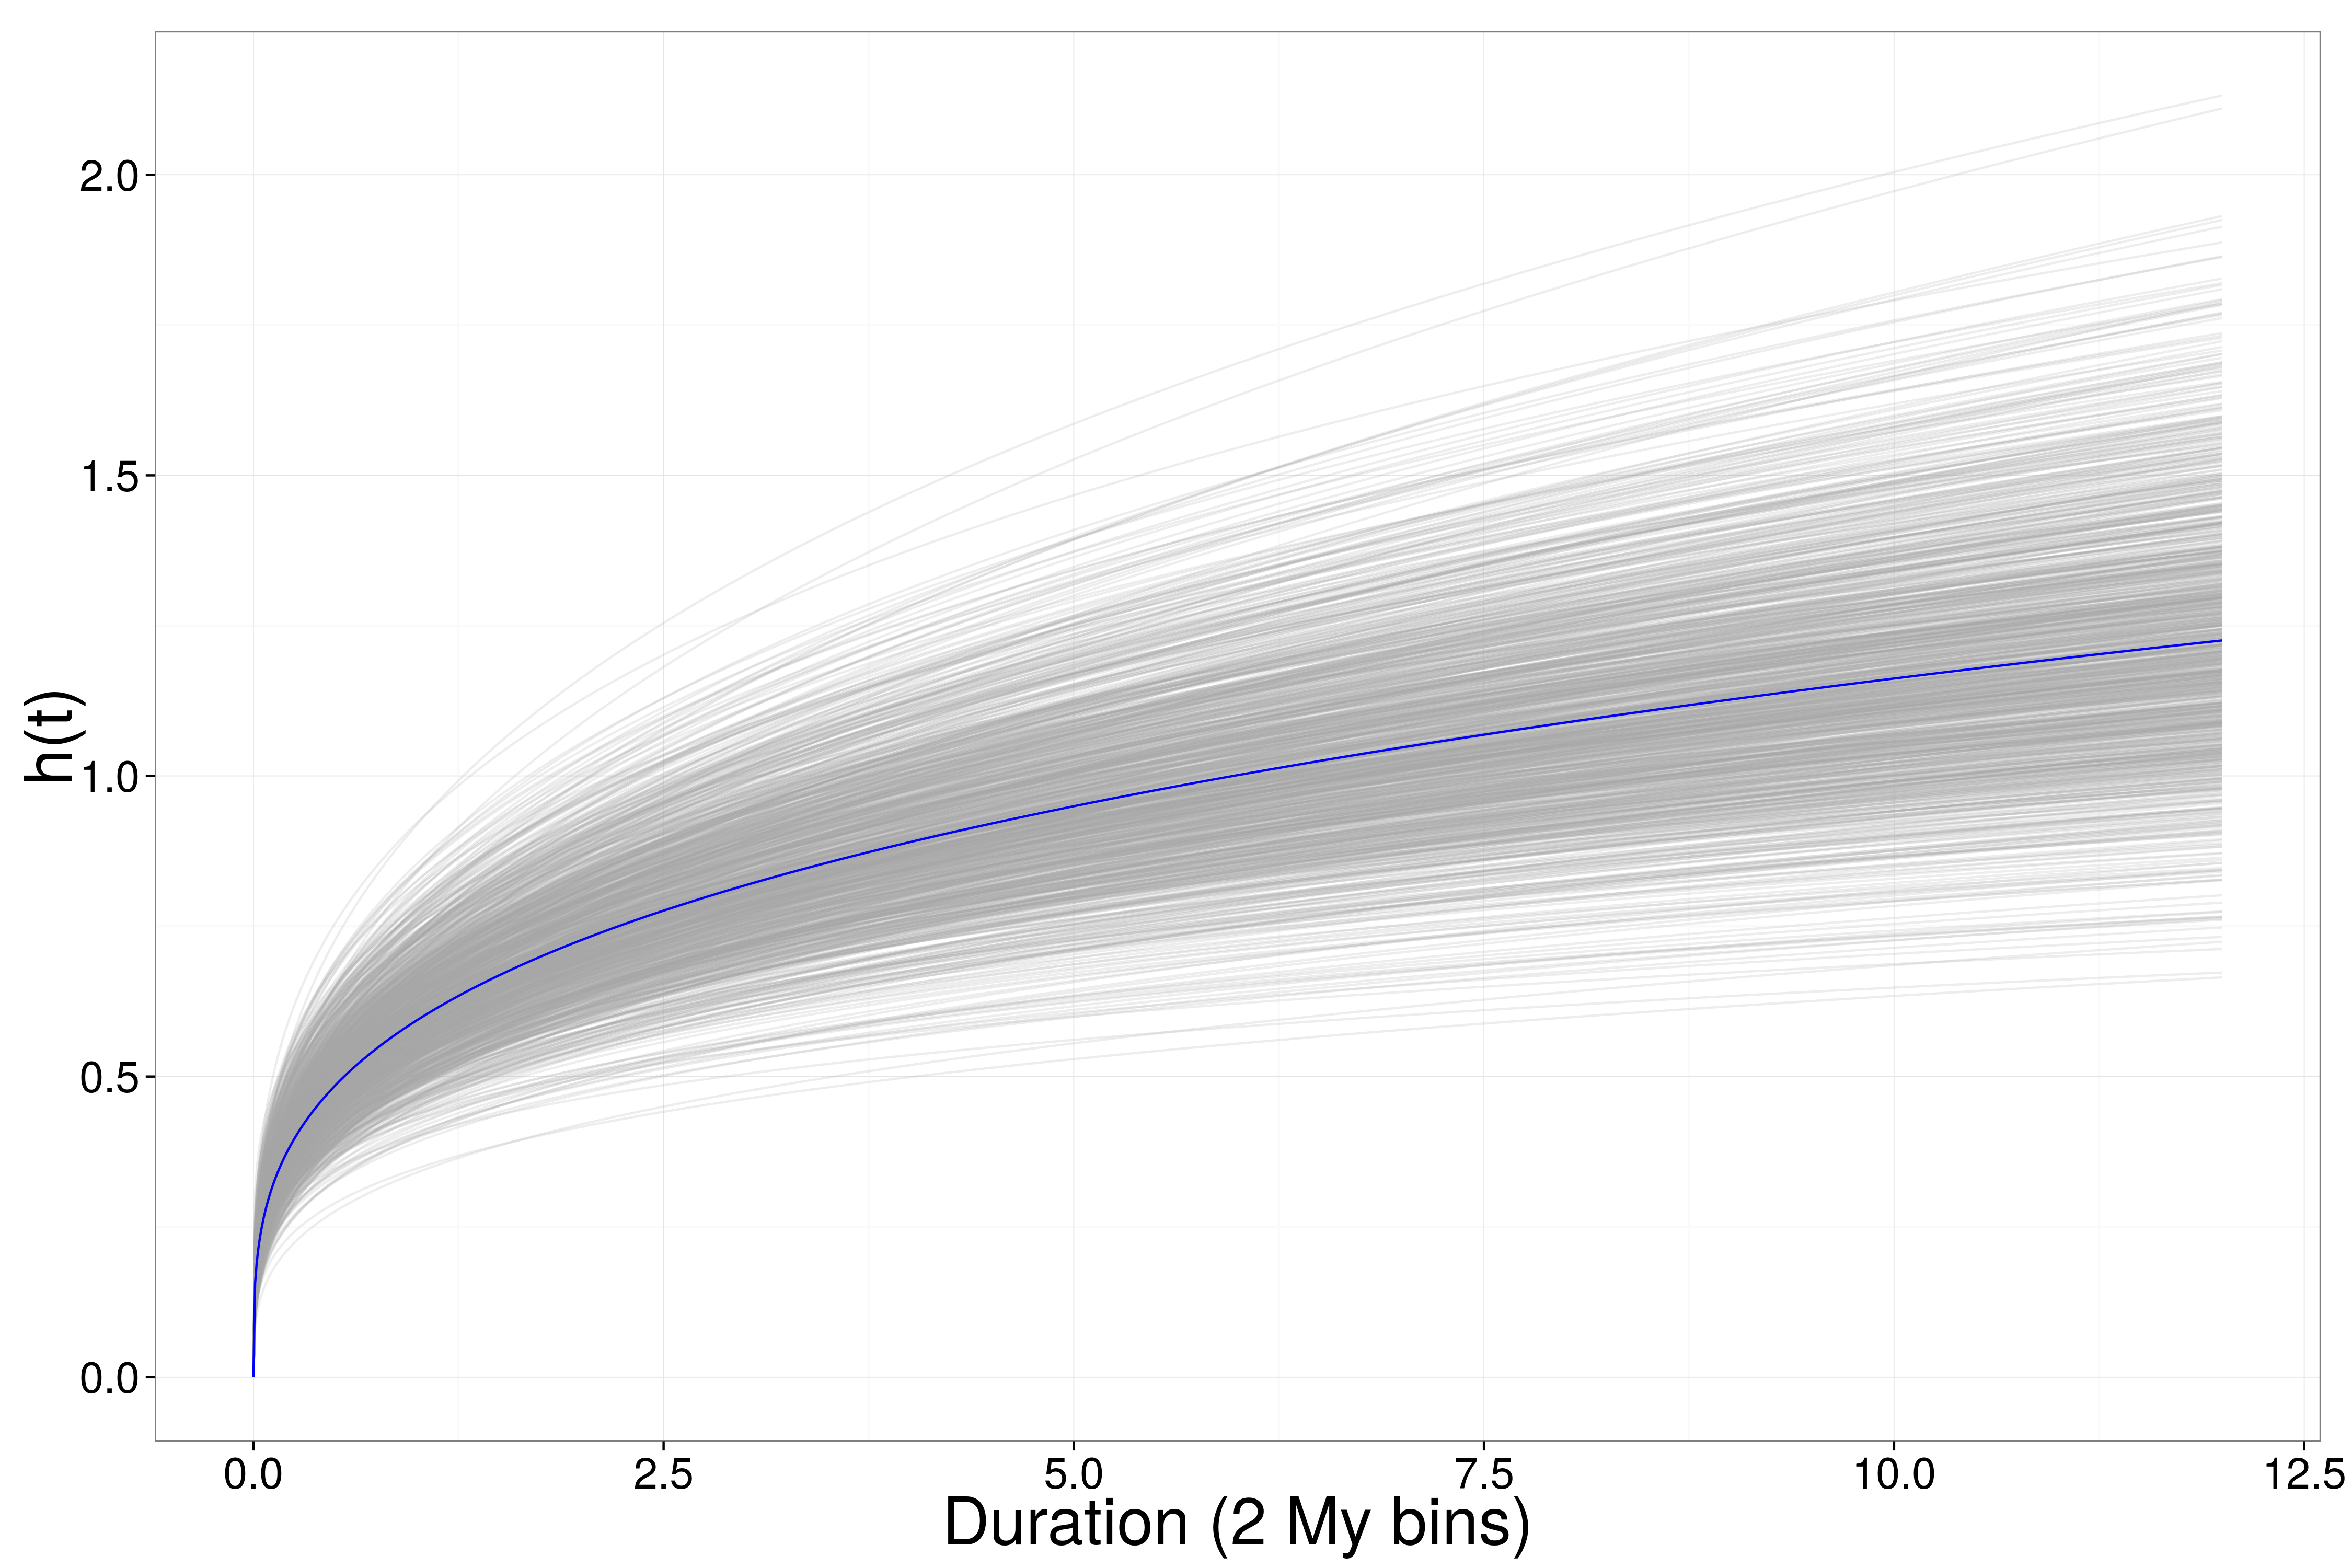
\includegraphics[height = 0.5\textheight, width = \textwidth, keepaspectratio = true]{figure/haz_est}
  \caption{1000 estimates of the hazard function (\(h(t\)) for the observed species mean (grey), along with the median estimated hazard function (blue). \(h(t)\) is an estimate of the rate at which a species of age \(t\) is expected to go extinct. Hazard functions were estimated from random draws from the estimated posterior distributions and evaluated with all covariate information set to 0, which corresponds to the expected duration of the mean species.}
  \label{fig:haz}
\end{suppfigure}
\clearpage
  
  
  
%\bibliographystyle{abbrvnat}
\bibliographystyle{pnas}
\bibliography{biblio}
  
  
\end{document}
